% ------------------- Aufgabe a -------------------
% R1: 67,23 \pm 0,1 (ohm)
% L: 16,87 \pm 0,05 (mH)
% positver Teil Parameter für Fit % y = a*exp(-b*x):
% a pos: 3.28805437898182 in V
% b pos: 4658.956201430903 in Hz
% negativer Teil Parameter für Fit % y = -a*exp(-b*x):
% a: 3.195407081244171 in V
% b neg: 4964.215848906855 in Hz
% R_eff_exp: 162.3+/-0.5 in ohm
% ------------------- Aufgabe b -------------------
% R_ap Theo: 5723+/-9 (ohm)
% ------------------- Aufgabe c -------------------
% Resonanzüberhöhung q theo: 4.226096298726022
% delta_omega theo: (4.043+/-0.012)e+04 in Hz
% delta_freq  theo(Breite der Resonanzkurve): 6434+/-20 in Hz
% Güte/Resonanzüberhöhung q theo: 4.196+/-0.008 in V
\section{Auswertung}
\label{sec:Auswertung}

\begin{figure}
  \centering
  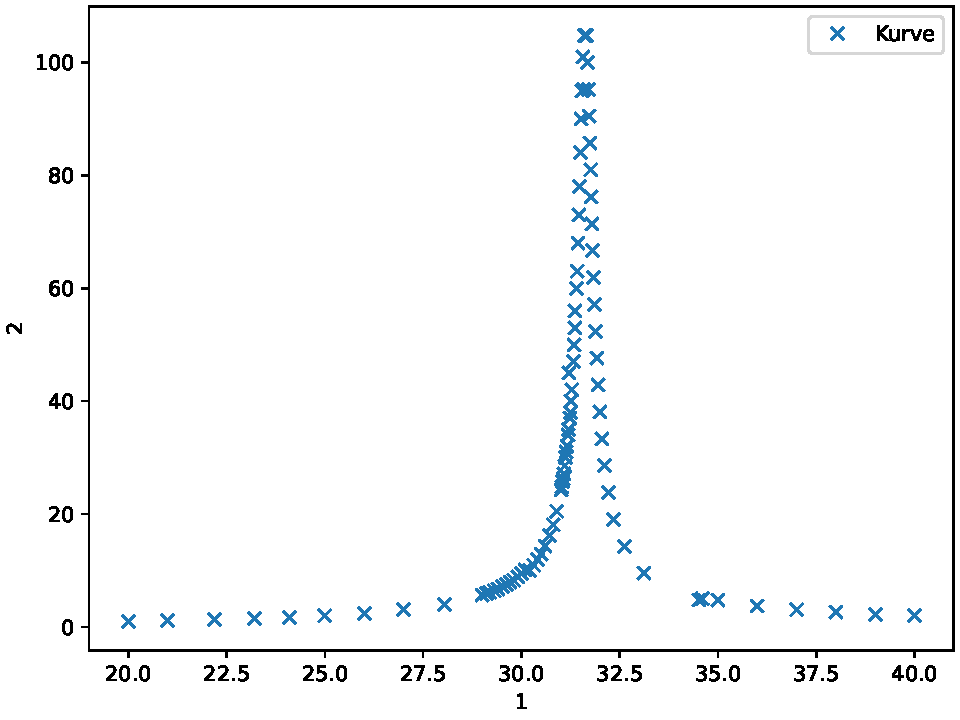
\includegraphics{plot.pdf}
  \caption{Plot.}
  \label{fig:plot}
\end{figure}

%Siehe \autoref{fig:plot}!